\chapter{理想光学系统}

\begin{introduction}
	\item 物像共轭关系(定义 \ref{def:conjugate})
	\item 基点和基面(第 \ref{subsect:base-point} 节)
	\item 光学系统的节点(第 \ref{subsect:nodal-points} 节)
	\item 光学系统的组合(第 \ref{sect:combination-of-optical-systems} 节)
	\item 光焦度(定义 \ref{def:focal-power})
	\item 视觉放大率(定义 \ref{def:visual-magnification})
\end{introduction}

将光学系统在近轴区完善成像的理论推广到任意大的空间,以任意宽的光束都成完善像的光学系统称为理想光学系统。共轴理想光学系统又称为高斯光学。

\section{理想光学系统与共线成像理论}

\begin{definition}{物像共轭关系}{conjugate}
	在理想光学系统中,任何一个物点发出的光线在系统的作用下所有的出射光线仍然相交于一点。由光路的可逆性和折射、反射定律中光线方向的确定性,可得出每一个物点对应于唯一一个像点。通常将这种物像对应关系叫做共轭。
\end{definition}

如果光学系统的物空间和像空间都是均匀透明介质,则入射光线和出射光线均为直线,根据光线的直线传播定律,由符合点对应点的物像空间关系可以推论出直线成像为直线、平面成像为平面的性质。这种点对应点、直线对应直线、平面对应平面的成像变换称为共线成像。

\begin{property}
共轴理想光学系统所成的像的性质:
\begin{enumerate}
	\item 位于光轴上的物点对应的共轭像点必然位于光轴上;位于过光轴的某一个截面内的物点对应的共轭像点必然位于该平面的共轭像面内;同时,过光轴的任意截面成像性质是相同的。
	\item 垂直于光轴平面物所成的共轭平面像的几何形状完全与物相似,在整个物平面上无论哪一部分,物和像的大小比例均等于常数。
	\item 一个共轴理想光学系统,如果已知两对共轭面的位置和放大率,或者一对共轭面的位置和放大率,以及轴上的两对共轭点的位置,则其他一切物点的像点都可以根据这些已知的共轭面和共轭点来表示。
\end{enumerate}
\end{property}

\section{理想光学系统的基点与基面}
\subsection{无限远轴上物点对应的像点}
\label{subsect:infty-object}

\begin{enumerate}	
	\item \textbf{无限远轴上物点发出的光线:}
	
	设$h$为轴上物点$A$发出的一条入射光线的投射高度,由三角关系近似有
	\begin{equation}
		\tan U=\frac{h}{L}
	\end{equation}
	式中,$U$为孔径角,$L$为物方截距。当$L$趋于无穷大时,物点$A$向无限远处左移,$U$趋于$0$,即无穷远轴上物点发出的光线都与光轴平行。
	\item \textbf{像方焦点、焦平面;像方主点、主平面:}
	
	如\figref{fig:perfect-optical-system} 所示,平行于光轴的入射光线$AE_1$通过理想光学系统后,出射光线$G'F'$交光轴于$F'$。$F'$为无限远轴上物点的像点,称为像方焦点。过$F'$作垂直于光轴的平面,称为像方焦平面。像方焦平面与无限远处垂直于光轴的物平面共轭。

	\begin{figure}[htbp]
		\centering
		\begin{tikzpicture} 
		\coordinate [label=above left:$O_1$] (A) at (-1,0);
		\coordinate [label=above right:$O_k$] (B) at (1,0);
		\coordinate [label=left:$A$] (C) at (-5,1.3);
		\coordinate [label=right:$A'$] (D) at (5,1.3);
		\coordinate [label=above:$Q'$] (E) at (-0.4,1.8);
		\coordinate [label=above:$Q$] (F) at (0.4,1.8);
		\coordinate [label=above:$F$] (G) at (-4,0);
		\coordinate [label=above:$F'$] (H) at (4,0);
		\coordinate [label=above left:$H'$] (I) at (-0.4,0);
		\coordinate [label=above right:$H$] (J) at (0.4,0);
		\coordinate (K) at (-0.4,1.3);
		\coordinate (L) at (0.4,1.3);
		\coordinate [label=above left:$E_1$] (M) at (-0.8,1.3);
		\coordinate [label=above right:$E_k$] (N) at (0.8,1.3);
		\coordinate [label=above left:$P$] (O) at (-0.8,0.8);
		\coordinate [label=above right:$G'$] (P) at (0.8,0.8);
		\draw[-] (-5,0) -- (5,0);
		\draw[-] (-5,1.3) -- (5,1.3);
		\draw[-] (-4,0) -- (-4,-1);
		\draw[-] (4,0) -- (4,-1.4);
		\draw[-latex] (C) -- (-3,1.3);
		\draw[-latex] (D) -- (3,1.3);
		\draw[-] (-0.4,1.8) -- (-0.4,-1.8);
		\draw[-] (0.4,1.8) -- (0.4,-1.8);
		\draw[latex-] (-4,0) -- (0.4,1.3);
		\draw[latex-] (4,0) -- (-0.4,1.3);
		\draw[line width=0.8pt] (A) arc (180:200:5);
		\draw[line width=0.8pt] (A) arc (180:160:5);
		\draw[line width=0.8pt] (B) arc (180:200:-5);
		\draw[line width=0.8pt] (B) arc (180:160:-5);
		\pic["$-u_1$", draw=black, -, angle eccentricity=1.6, angle radius=0.8cm] {angle=A--G--L};
		\pic["$u'_k$", draw=black, -, angle eccentricity=1.6, angle radius=0.8cm] {angle=K--H--B};
		\draw[latex-latex](-4,-0.8) -- (0.4,-0.8) node[black,below,midway](line){$-f$};
		\draw[latex-latex](4,-1.2) -- (-0.4,-1.2) node[black,below,midway](line){$f'$};
		\draw[latex-latex] (-4.5,1.3) -- ($(A)!(-4.5,1.3)!(B)$)node[black,midway,xshift=0.2cm]{$h_1$};
		\end{tikzpicture}
		\caption{理想光学系统}
		\label{fig:perfect-optical-system}
	\end{figure}
	
	入射光线$AE_1$的延长线与出射光线$G'F'$的反向延长线交于一点$Q'$,过$Q'$作垂直于光轴的平面交光轴于$H'$点,则$H'$点为像方主点,$Q'H'$平面为像方主平面,从主点$H'$搭配焦点$F'$之间的距离为像方焦距$f'$。有
	\begin{equation}
		f'=\frac{h}{\tan U'}
	\end{equation}
	
	\item \textbf{无限远轴外物点发出的光线:}
	
	进入光学系统的光线总是相互平行的,且与光轴有一定夹角$\omega$。这一束光线经过系统后,一定交于像方焦平面的某一点,这一点为无限远轴外物点的共轭像点。	
\end{enumerate}

\subsection{无限远轴上像点对应的物点}
相关概念同第 \ref{subsect:infty-object} 节内容。物方焦平面上任意一点发出的光线,通过理想光学系统后亦是一组相互平行的光线。

\begin{figure}[htbp]
	\centering
	\includegraphics[width=0.6\textwidth]{lens-shapes.pdf}
	\caption{不同形状透镜的主平面}
	\label{fig:lens-shapes}
\end{figure}

\subsection{物方主平面与像方主平面}
\label{subsect:base-point}
如\figref{fig:perfect-optical-system} 所示,两条入射光线$AE_1$和$FP$都经过$Q$,相应地出射光线都经过$Q'$,$Q$和$Q'$为共轭点,因此物方主平面和像方主平面是一对共轭面,垂轴放大率为$+1$。不同形状透镜的主平面位置如\figref{fig:lens-shapes} 所示。对于此类厚透镜的主面位置分析见第 \ref{subsect:thick-lenses} 节。

\begin{definition}{基点和基面}{base-point}
	一对主点和主平面,一对焦点和焦平面,称为共轴理想光学系统的基点和基面。
\end{definition}

\section{理想光学系统的物像关系}
\subsection{牛顿公式}

\begin{figure}[htbp]
	\centering
	\begin{tikzpicture} 
	\coordinate [label=above left:$Q$] (A) at (-0.4,1.2);
	\coordinate [label=above right:$Q'$] (B) at (0.4,1.2);
	\coordinate [label=above left:$A$] (C) at (-4,0);
	\coordinate [label=above right:$A'$] (D) at (4,0);
	\coordinate [label=above left:$H$] (E) at (-0.4,0);
	\coordinate [label=above right:$H'$] (F) at (0.4,0);
	\coordinate [label=left:$B$] (G) at (-4,1.2);
	\coordinate [label=right:$B'$] (H) at (4,-1.6);
	\coordinate [label=above left:$R$] (I) at (-0.4,-1.2);
	\coordinate [label=above right:$R'$] (J) at (0.4,-1.2);
	\coordinate [label=below right:$R_1$] (K) at (-0.4,-1.6);
	\coordinate [label=above:$F$] (L) at (-2.455,0);
	\coordinate [label=above:$F'$] (M) at (1.95,0);
	\coordinate [label=right:$y$] (N) at (-4,0.6);
	\coordinate [label=right:$-y'$] (O) at (4,-0.8);
	\coordinate (L) at (0.4,-1.6);
	\draw[-] (-5,0) -- (5,0);
	\draw[-] (-0.4,1.6) -- (-0.4,-2.5);
	\draw[-] (0.4,1.6) -- (0.4,-2.5);
	\draw[-] (C) -- (A);
	\draw[-] (D) -- (B);
	\draw[-,dashed] (A) -- (B);
	\draw[-,dashed] (I) -- (J);
	\draw[-,dashed] (K) -- (L);
	\draw[-] (G) -- (A);
	\draw[-] (B) -- (H);
	\draw[-] (C) -- (I);
	\draw[-] (J) -- (D);
	\draw[-] (G) -- (K);
	\draw[-] (L) -- (H);
	\draw[-] (-4,0) -- (-4,-2.5);
	\draw[-] (4,-1.6) -- (4,-2.5);
	\draw[-] (-2.455,0) -- (-2.45,-2);
	\draw[-] (1.95,0) -- (1.95,-2);
	\draw[-latex,red,line width=1.2pt] (C) -- (G);
	\draw[-latex,red,line width=1.2pt] (D) -- (H);
	\draw[latex-latex](-4,-1.8) -- (-2.455,-1.8) node[black,below,midway](line){$-x$};
	\draw[latex-latex](-0.4,-1.8) -- (-2.455,-1.8) node[black,below,midway](line){$-f$};
	\draw[latex-latex](4,-1.8) -- (1.95,-1.8) node[black,below,midway](line){$x'$};
	\draw[latex-latex](0.4,-1.8) -- (1.95,-1.8) node[black,below,midway](line){$f'$};
	\draw[latex-latex](-4,-2.3) -- (-0.4,-2.3) node[black,below,midway](line){$-l$};
	\draw[latex-latex](4,-2.3) -- (0.4,-2.3) node[black,below,midway](line){$l'$};
	\pic["$-u$", draw=black, -, angle eccentricity=1.4, angle radius=0.6cm] {angle=D--C--A};
	\pic["$u'$", draw=black, -, angle eccentricity=1.4, angle radius=0.6cm] {angle=B--D--C};
	\end{tikzpicture}
	\caption{物像位置}
	\label{fig:newton-and-gauss}
\end{figure}

如\figref{fig:newton-and-gauss} 所示,由相似三角形可导出
\begin{equation}
xx'=ff'
\label{eq:newton-eq-1}
\end{equation}
\begin{equation}
\beta=\frac{y'}{y}=-\frac{x'}{f'}=-\frac{f}{x}
\label{eq:newton-eq-2}
\end{equation}
式(\ref{eq:newton-eq-1})为牛顿公式,以焦点为原点。式(\ref{eq:newton-eq-2})为牛顿公式的垂轴放大率公式。

\subsection{高斯公式}
如\figref{fig:newton-and-gauss} 所示,焦物距、焦像距和物距、像距之间有如下关系:
\begin{equation}
x=l-f,\quad x'=l'-f'
\end{equation}
将其带入牛顿公式(\ref{eq:newton-eq-1}),两边同时除以$ll'$可得
\begin{equation}
\frac{f'}{l'}+\frac{f}{l}=1
\label{eq:gauss-eq-1}
\end{equation}
式(\ref{eq:gauss-eq-1})为高斯公式,以主点为原点。其相应的垂轴放大率公式为
\begin{equation}
\beta=\frac{y'}{y}=-\frac{f}{f'}\frac{l'}{l}
\label{eq:gauss-eq-2}
\end{equation}
当物方介质和像方介质相同时,有$f'=-f$,则式(\ref{eq:gauss-eq-1})和式(\ref{eq:gauss-eq-2})可以写成
\begin{equation}
\frac{1}{l'}-\frac{1}{l}=\frac{1}{f'}
\end{equation}
\begin{equation}
\beta=\frac{l'}{l}
\end{equation}

\subsection{两焦距之间的关系}
在近轴光线区域,$fyu=-f'y'u'$,共轴球面系统的近轴区适用拉赫公式$nyu=n'y'u'$,则可得出物方焦距和像方焦距之间的关系式:
\begin{equation}
\frac{f'}{f}=-\frac{n'}{n}
\end{equation}
若光学系统中包括反射面,则两焦距之间的关系由反射面个数决定。设反射面个数为$k$,则有
\begin{equation}
\frac{f'}{f}=(-1)^{k+1}\frac{n'}{n}
\end{equation}
理想光学系统的拉赫公式为
\begin{equation}
ny\tan U=n'y'\tan U'
\label{eq:lah-eq}
\end{equation}

\section{理想光学系统的放大率}
前面已经给出垂轴放大率的公式(\ref{eq:newton-eq-2})和(\ref{eq:gauss-eq-2}),下面给出轴向放大率和角放大率。
\subsection{轴向放大率}
物平面沿光轴移动$\mathrm{d} x$或$\mathrm{d} l$时,像平面移动$\mathrm{d} x'$或$\mathrm{d} l'$,轴向放大率为
\begin{equation}
\alpha=\frac{\mathrm{d} x'}{\mathrm{d} x}=\frac{\mathrm{d} l'}{\mathrm{d} l}
\end{equation}
微分可得
\begin{equation}
\alpha=-\frac{x'}{x}
\end{equation}
将式(\ref{eq:newton-eq-2})带入得
\begin{equation}
\alpha=-\beta^2\frac{f'}{f}=\frac{n'}{n}\beta^2
\end{equation}

\subsection{角放大率}
角放大率为
\begin{equation}
\gamma=\frac{\tan U'}{\tan U}
\end{equation}
根据理想光学系统拉赫公式(\ref{eq:lah-eq})得
\begin{equation}
\gamma=\frac{n}{n'}\frac{1}{\beta}
\end{equation}
理想光学系统三种放大率之间的关系为
\begin{equation}
\alpha\gamma=\beta
\end{equation}

\begin{problem}
	物方、像方介质相同的光学系统对物成像,当$\alpha<1$时,有:
	\begin{tasks}(2)
		\task 物像同向移动,像移动的速度比物快
		\task 物像同向移动,像移动的速度比物慢
		\task 成放大像
		\task 成缩小像
	\end{tasks}
\end{problem}
\begin{solution}
	选择b和d。
\end{solution}

\begin{problem}
	某物方、像方介质相同的折射光学系统对物成像时有$-1<\beta<0$,则当物体向透镜移动时有:
	\begin{tasks}(2)
		\task 像向透镜移动
		\task 像远离透镜移动
		\task 像移动速度比物快
		\task 像移动速度比物慢
	\end{tasks}
\end{problem}
\begin{solution}
	选择b和d。
\end{solution}

\begin{problem}
	无穷远物通过透镜成像放大率为$0$,是否只是一个点?
\end{problem}
\begin{solution}
	并非如此,放大率为$0$只是物在无穷远时公式的计算结果,但实际上并不是一个点。反过来思考:位于焦平面上的物体,成像在无穷远。
\end{solution}

\subsection{光学系统中的节点}
\label{subsect:nodal-points}

\begin{definition}{节点}{nodal-points}
	光学系统中角放大率等于$+1^{\times}$的一对共轭点为节点。厚透镜的节点位置如\figref{fig:nodal-points} 所示
\end{definition}

\begin{property}
	光线通过节点方向不发生改变。
\end{property}

\begin{problem}
	正透镜对虚物成像时:
	\begin{tasks}(4)
		\task 只能成实像
		\task 只能成虚像
		\task 只能成缩小像
		\task 只能成放大像
	\end{tasks}
\end{problem}

\begin{solution}
	选择a和c。
\end{solution}

\begin{problem}
	光学系统的节点是:
	\begin{tasks}(2)
		\task 垂轴放大率为$1$的共轭点
		\task 角放大率为$1$的共轭点
		\task 物方发出过物方节点的光必经过像方节点
		\task 物方发出过像方节点的光必经过物方节点
	\end{tasks}
\end{problem}

\begin{solution}
	选择b和c。
\end{solution}

\begin{figure}[htbp]
	\centering
	\begin{minipage}[t]{0.3\textwidth}
		\centering
		\begin{tikzpicture} [scale=0.87 ] 
		\coordinate (A) at (-1,0);
		\coordinate (B) at (1,0);
		\coordinate [label=above:$N$] (C) at (-0.5,0);
		\coordinate [label=below:$N'$] (D) at (0.5,0);
		\coordinate (E) at (-2,0);
		\coordinate (F) at (2,0);
		\coordinate (G) at (-2,-2);
		\coordinate (H) at (2,2);
		\draw[-,dashed] (E) -- (F);
		\draw[-,dashed,red,name path=pathA] (G) -- (C);
		\draw[-,dashed,red,name path=pathB] (H) -- (D);
		\draw[line width=0.8pt,name path=pathC] (A) arc (180:200:5);
		\draw[line width=0.8pt] (A) arc (180:160:5);
		\draw[line width=0.8pt,name path=pathD] (B) arc (180:200:-5);
		\draw[line width=0.8pt] (B) arc (180:160:-5);
		\path [name intersections={of = pathA and pathC, by=I}];
		\path [name intersections={of = pathB and pathD, by=J}];
		\draw[-,red] (I) -- (J);
		\draw[-latex,red] (G) -- (I);
		\draw[-latex,red] (J) -- (H);
		\pic["$\theta$", draw=black, -, angle eccentricity=1.2, angle radius=1cm] {angle=E--C--G};
		\pic["$\theta$", draw=black, -, angle eccentricity=1.2, angle radius=1cm] {angle=F--D--H};
		\end{tikzpicture}
		\caption{厚透镜的节点}
		\label{fig:nodal-points}
	\end{minipage}
	\quad
	\begin{minipage}[t]{0.6\textwidth}
		\centering
		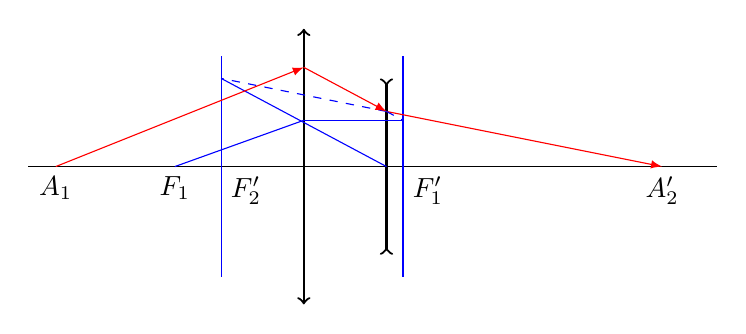
\begin{tikzpicture} [scale=0.7] 
		\draw[-] (-6.5,0) -- (6,0); 
		\draw[<->,line width=0.8pt] (-1.5,2.5) -- (-1.5,-2.5); 
		\draw[>-<,line width=0.8pt] (0,1.6) -- (0,-1.6); 
		\draw[-,blue] (-3,2) -- (-3,-2);
		\draw[-,blue] (0.3,2) -- (0.3,-2);
		\draw[-latex,red] (0,1) -- (5,0);
		\draw[-,dashed,blue] (0,1) -- (-3,1.6);
		\draw[-,dashed,blue] (0,1) -- (0.3,0.84);
		\draw[-,blue] (0,0) -- (-3,1.6);
		\draw[latex-,red] (0,1) -- (-1.5,1.8);
		\draw[-,blue] (0.3,0.84) -- (-1.5,0.84);
		\draw[-,blue] (-3.84,0) -- (-1.5,0.84);
		\draw[-latex,red] (-6,0) -- (-1.5,1.8);
		\coordinate [label=below:$A_1$] (A) at (-6,0);
		\coordinate [label=below:$F_1$] (B) at (-3.84,0);
		\coordinate [label=below right:$F'_2$] (C) at (-3,0);
		\coordinate [label=below right:$F'_1$] (D) at (0.3,0);
		\coordinate [label=below:$A'_2$] (E) at (5,0);
		\end{tikzpicture}
		\caption{图解求像}
		\label{fig:draw-beam-path}
	\end{minipage}
\end{figure}

\section{理想光学系统的图解求像}
画光路图的依据:
\begin{enumerate}
	\item 平行于光轴的光线经理想光学系统后必通过像方焦点;
	\item 过物方焦点的光线经理想光学系统后必为平行于光轴的光线;
	\item 过节点的光线方向不变;
	\item 任意方向的一束平行光经理想光学系统后必交于像方焦平面上一点;
	\item 过物方焦平面上一点的光线经理想光学系统后必为一束平行光;
	\item 主面交点光线高度相同。
\end{enumerate}

\begin{exercise}
	如\figref{fig:draw-beam-path} 所示,已知二光组基点,由物求像或由像求物。
\end{exercise}

\begin{note}
	在这一类绘制光路图的题中,需要注意过第二个透镜光轴处的辅助线与过第一个透镜到其焦面$F_1$的光线平行,这一条线要交于第二个透镜的焦面$F_2$处,经过该交点与光线和第二个透镜的交点的线即为出射光线。图解求像是考试中必考的题目。在大二学习这部分内容的时候,期中考试因为作图题扣了很多分。这一类的题需要多练,如果熟练掌握的话,完全是送分题,否则就是送命题。
\end{note}

\section{理想光学系统的组合}
\label{sect:combination-of-optical-systems}
\begin{figure}[htbp]
	\centering
	\includegraphics[width=1\textwidth]{combination-of-optical-systems.png}
	\caption{两个光组的组合}
	\label{fig:combination-of-optical-systems}
\end{figure}

\figref{fig:combination-of-optical-systems} 给出了由两个光组组成的等效系统在两个空间的焦点和主点。按牛顿公式,物焦距$x=-\varDelta$,其焦像距$x'_F$为
\begin{equation}
x'_F=-\frac{f_2f'_2}{\varDelta}
\end{equation}
同理有
\begin{equation}
x_F=\frac{f_1f'_1}{\varDelta}
\end{equation}
根据相似三角形$\triangle Q'H'F'\sim\triangle N'_2H'_2F'_2$、$\triangle Q'_1H'_1F'_1\sim\triangle E_2F_2F'_1$,可导出
\begin{equation}
f'=-\frac{f'_1f'_2}{\varDelta}
\label{eq:combination-of-optical-systems-focal-length}
\end{equation}
同理有
\begin{equation}
f=\frac{f_1f_2}{\varDelta}
\end{equation}
大多数情况下光学系统位于空气中,应有$f'_1=-f_1$,$f'_2=-f_2$和$f'=-f$。所以有
\begin{equation}
\varDelta=d-f'_1+f_2=d-f'_1-f'_2
\end{equation}
则有
\begin{equation}
f'=-f=\frac{f'_1f'_2}{f'_1+f'_2-d}
\end{equation}
表示成光焦度形式为
\begin{equation}
\varphi=\varphi_1+\varphi_2-d\varphi_1\varphi_2
\end{equation}

\begin{definition}{折合距离与光焦度}{focal-power}
	一线段的长度除以该线段所在介质的折射率做得的值称为该线段的折合距离。折合焦距的倒数称之为光学系统的光焦度,以$\varPhi$表示,即
	\begin{equation}
	\varPhi=\frac{n'}{f'}=-\frac{n}{f}
	\end{equation}
	如果光学系统位于空气中,其光焦度用$\varphi$表示,即
	\begin{equation}
	\varphi=\frac{1}{f'}=-\frac{1}{f}
	\end{equation}
	光焦度的单位是折光度或屈光度。正光焦度的光学系统对光束起会聚作用;负光焦度的光学系统对光束起发散作用。
\end{definition}

根据\figref{fig:combination-of-optical-systems},还可得到如下关系:
\begin{equation}
\begin{cases}
l'_F=f'_2+x'_F,\quad l_F=f_1+x_F\\
l'_H=l'_F-f',\quad l_H=l_F-f
\end{cases}
\end{equation}
据此可得出等效系统基点相对于主点的位置关系。

等效系统的放大率$\beta$仍可用基本公式$\beta=-f/x$计算。$f$为等效系统的焦距,$x$为物点到等效系统的物方焦点距离,得到
\begin{equation}
\beta=\frac{f_1f_2}{f_1f'_1-x_1\varDelta}
\end{equation}

\begin{problem}
	空气中两光组组合的光焦度公式,如果物方像方或两光组之间的介质不是空气,公式是否会变化,怎么变化,为什么?
\end{problem}
\begin{solution}
	设物方介质折射率为$n_1$,两光组之间折射率为$n_2$,像方折射率为$n_3$。有
	\begin{equation}
	\varDelta=d-f'_1+f_2\notag
	\end{equation}
	\begin{equation}
	f'=\frac{-f'_1f'_2}{\varDelta}\notag
	\end{equation}
	由
	\begin{equation}
	\frac{f'_2}{n_3}=-\frac{f_2}{n_2}\notag
	\end{equation}
	得到
	\begin{equation}
	f'=\frac{f'_1f'_2}{f'_1+\dfrac{n_2}{n_3}f'_2-d}\notag
	\end{equation}
	又有
	\begin{equation}
	\varphi=\frac{n_3}{f'},\quad\varphi_1=\frac{n_2}{f'_1},\quad\varphi_2=\frac{n_3}{f'_2}\notag
	\end{equation}
	所以,光焦度的表达式为
	\begin{equation}
	\varphi=\varphi_2+\varphi_2-\frac{d\varphi_1\varphi_2}{n_2}\notag
	\end{equation}
	由此可知,光焦度与物方像方介质无关,与两光组之间的介质有关。
\end{solution}

\begin{problem}
	一短焦距广角照相物镜的焦距$f'=28\mathrm{mm}$,工作距离$l'_F=40\mathrm{mm}$,总长度(第一透镜到物镜像方焦点的距离)$L=55\mathrm{mm}$,求组成此系统的两个薄透镜的焦距$f'_1$,$f'_2$以及其间隔$d$。
\end{problem}

\begin{problem}
	有一双透镜系统,已知$f'_1=100\mathrm{mm}$,$f'_2=-50\mathrm{mm}$,要求总长度为系统焦距的$0.7$倍,求两透镜的间隔和系统的焦距。
\end{problem}

\begin{problem}
	人眼可简化成一曲率半径为$5.6\mathrm{mm}$的单个折射球面,其像方折射率为$4/3$。求远处对眼睛张角为$1^{\circ}$的物体在视网膜上所成像的大小。
\end{problem}

\section{望远镜系统}

\begin{definition}{望远镜系统}{telescope}
	使入射的平行光束仍保持平行地出射的光学系统称为望远镜系统。望远镜系统的焦距无穷大,焦点和主点位于无穷远。
\end{definition}

\begin{figure}[htbp]
	\centering
	\includegraphics[width=0.7\textwidth]{telescope-system.png}
	\caption{望远镜系统}
	\label{fig:telescope-system}
\end{figure}

如\figref{fig:telescope-system} 所示,根据牛顿公式,并考虑过渡公式$\varDelta=0$,可导出
\begin{equation}
x'_2=\frac{f_2f'_2}{f_1f'_1}x_1
\end{equation}
\begin{equation}
\beta=\beta_1\beta_2=\frac{f_2}{f'_1}
\end{equation}
轴向放大率公式为
\begin{equation}
\alpha=\frac{\mathrm{d}x'_2}{\mathrm{d}x_1}=\frac{f_2f'_2}{f_1f'_1}
\end{equation}
角放大率为
\begin{equation}
\gamma=\frac{\tan u'}{\tan u}=\frac{f_1}{f_2}
\end{equation}
在空气中,$f'_1=-f_1$,$f'_2=-f_2$,因此有
\begin{equation}
\beta=-\frac{f'_2}{f'_1}
\end{equation}
\begin{equation}
\alpha=\beta^2
\end{equation}
\begin{equation}
\gamma=-\frac{f'_1}{f'_2}=\frac{1}{\beta}
\end{equation}
\begin{equation}
x'_2=\alpha x_1
\end{equation}
由此可见,望远镜系统的各种放大率,仅由组成该系统的两个光组的焦距决定。

供眼睛观察用的光学系统为目视光学系统,目视光学系统中最重要的参数为视觉放大率。
\begin{definition}{视觉放大率}{visual-magnification}
	望远镜系统的视觉放大率是远处物体经系统所成的像对眼睛张角$W'$的正切与该物体直接对眼睛张角$W$的正切之比,用$\varGamma$表示。望远镜系统的视觉放大率等于该系统的角放大率,即
	\begin{equation}
	\varGamma=\frac{\tan W'}{\tan W}=\gamma=-\frac{f'_1}{f'_2}=\frac{1}{\beta}
	\end{equation}
	所以,望远镜系统的视觉放大率是物镜焦距与目镜焦距之比。
\end{definition}

一个有限焦距系统之前加角放大率为$\varGamma$的望远镜系统时,整个系统的焦距为原焦距的$\varGamma$倍,即
\begin{equation}
f'=\varGamma f'_2
\end{equation}

\begin{problem}
	开普勒望远镜系统,物方视场增大到一定程度就看不到像了,为什么在物镜和目镜之间加个透镜又能看到像了?这个透镜应该加在何处?
\end{problem}
\begin{solution}
	物方视场增大到一定程度后,折射角仍然过大,光线被拦,所以无法成像。在中间加个透镜,光束会聚,使原本被拦的光线通过,因此可以重新看到像。该透镜为场镜,加在中间的实像面上。
\end{solution}

\begin{problem}
	当物镜焦距大于目镜焦距时,望远镜成放大像还是缩小像?眼睛看到的是放大像还是缩小像?为什么?
\end{problem}
\begin{solution}
	由$\beta=-f'_2/f'_1$可知,$|\beta|<1$,望远镜成缩小像,而$\gamma=1/\beta$,$|\gamma|>1$,视觉放大率大于$1$,眼睛看到的是放大像。
\end{solution}

\begin{problem}
	某望远镜物镜由正、负分离的两个薄透镜组组成,已知$f'_1=500\mathrm{mm}$,$f'_2=-400\mathrm{mm}$,$d=300\mathrm{mm}$,求其焦距。若用此望远镜来观察前方$200\mathrm{mm}$处的物体时,仅用第二个负透镜组来调焦以使其像仍位于物镜的原始焦平面上,问该镜组应向什么方向移动多少距离?此时物镜的焦距为多少?
\end{problem}

\begin{problem}
	\begin{figure}[htbp]
		\centering
		\includegraphics[width=0.5\textwidth]{telescope-objective.png}
		\caption{双胶合望远镜物镜}
		\label{fig:telescope-objective}
	\end{figure}
	如\figref{fig:telescope-objective} 所示的双胶合望远镜物镜,按如下要求分别计算组合系统的焦距和像方基点的位置。
	\begin{enumerate}[(1)]
		\item 在双胶合物镜前加一视觉放大率$\Gamma=-8$的望远镜系统;
		\item 在双胶合物镜前加一视觉放大率$\Gamma=3$的望远镜系统;
		\item 在双胶合物镜后加一厚度为$60\mathrm{mm}$,折射率为$1.5$的平行平板。
	\end{enumerate}
\end{problem}

\section{透镜}
\subsection{薄透镜}

\begin{definition}{薄透镜}{thin-lens}
	透镜的厚度与球面半径相比很小,略去厚度不会引起成像结果的实质性变化,却能对初始阶段的分析和计算带来方便,导出简单的公式。这时认为透镜的厚度为零,称薄透镜。
\end{definition}

薄透镜的物像位置公式:
\begin{equation}
\frac{1}{l'}-\frac{1}{l}=(n-1)\bigg(\frac{1}{r_1}-\frac{1}{r_2}\bigg)
\label{eq:thin-lens}
\end{equation}
焦距为
\begin{equation}
f'=\frac{1}{(n-1)\bigg(\dfrac{1}{r_1}-\dfrac{1}{r_2}\bigg)}
\end{equation}
并有$f=-f'$。其光焦度为
\begin{equation}
\varphi=\frac{1}{f'}=(n-1)\bigg(\frac{1}{r_1}-\frac{1}{r_2}\bigg)
\end{equation}
则式(\ref{eq:thin-lens})可以写成
\begin{equation}
\frac{1}{l'}-\frac{1}{l}=\frac{1}{f'}=\varphi
\end{equation}

由此可知,凸透镜焦距为正,光焦度为正,对光束起会聚作用,像方焦点是对入射平行光束会聚而成的实焦点。凹透镜焦距为负,光焦度为负,对光束起发散作用,像方焦点为虚焦点。因此称凸透镜为正透镜或会聚透镜,凹透镜为负透镜或发散透镜。

通过
\begin{equation}
\beta=\frac{f'}{l+f'}
\end{equation}
可以得出,当$\beta=1$时,解得$l=0$,此时一对物像点重合于薄透镜的中心或顶点,角放大率为$1$,表示这一对共轭点共轭光线有相同方向。因这对共轭点重合于薄透镜中心,所以过薄透镜中心的光线方向不变。

\begin{property}
	薄透镜具有下列性质:
\begin{enumerate}
	\item 平行于光轴入射的光线经透镜后通过像方焦点;
	\item 过物方焦点的入射光线经过透镜后平行于光轴射出;
	\item 通过透镜中心的光线方向不变。
\end{enumerate}
\end{property}

\begin{problem}
	一个$f'=80\mathrm{mm}$的薄透镜当物体位于其前何处时,正好能在透镜前$250\mathrm{mm}$处成像?
	\begin{tasks}(2)
		\task 位于其前$60.6\mathrm{mm}$
		\task 位于其前$117.6\mathrm{mm}$
		\task 位于其后$60.6\mathrm{mm}$
		\task 位于其后$117.6\mathrm{mm}$
	\end{tasks}
\end{problem}
\begin{solution}
	选择a。
\end{solution}

\begin{problem}
	以下光学系统中,对实物一定成虚像的是:
	\begin{tasks}(4)
		\task 反射球面
		\task 平行平板
		\task 负薄透镜
		\task 正薄透镜
	\end{tasks}
\end{problem}
\begin{solution}
	选择b和c。
\end{solution}

\begin{problem}
	单薄透镜成像时,若共轭距(物与像之间的距离)为$250\mathrm{mm}$,求下列情况下透镜应有的焦距:(1) 实物,$\beta=-4$;(2) 实物,$\beta=-1/4$;(3) 虚物,$\beta=-4$;(4) 实物,$\beta=4$;(5) 虚物,$\beta=4$。
\end{problem}
\begin{solution}
	薄透镜的物像位置关系公式为
	\begin{equation}
	\frac{1}{l'}-\frac{1}{l}=\frac{1}{f'}, \quad \beta=\frac{l'}{l} \nonumber
	\end{equation}
	共轭距为
	\begin{equation}
	l'-l=250\mathrm{mm} \nonumber
	\end{equation}
	所以
	\begin{enumerate}[(1)]
		\item 实物,$\beta=-4$。$l'=200\mathrm{mm}$,$l=-50\mathrm{mm}$,$f'=40\mathrm{mm}$。
		\item 实物,$\beta=-1/4$。$l'=50\mathrm{mm}$,$l=-200\mathrm{mm}$,$f'=40\mathrm{mm}$。
		\item 虚物,$\beta=-4$。$l'=-200\mathrm{mm}$,$l=50\mathrm{mm}$,$f'=-40\mathrm{mm}$。
		\item 实物,$\beta=4$。$l'=-1000/3\mathrm{mm}$,$l=-250/3\mathrm{mm}$,$f'=111.11\mathrm{mm}$。
		\item 虚物,$\beta=4$。$l'=1000/3\mathrm{mm}$,$l=250/3\mathrm{mm}$,$f'=-111.11\mathrm{mm}$。
	\end{enumerate}
\end{solution}

\begin{problem}
	用135照相机(物镜的焦距为$50\mathrm{mm}$)拍照时,若要求对身高为$1.7\mathrm{mm}$的人在底片上获得$17\mathrm{mm}$高的像,物镜相对于焦平面的调焦量应为多少?人大致离照相机多少距离?
\end{problem}
\begin{solution}
	由牛顿公式
	\begin{equation}
	\beta=\frac{y'}{y}=-\frac{x'}{f'} \Rightarrow \frac{-17}{1700}=-\frac{x'}{50}\nonumber
	\end{equation}
	得$x'=0.5\mathrm{mm}$;由
	\begin{equation}
	\frac{1}{l'}-\frac{1}{l}=\frac{1}{f'}, \quad \beta=\frac{l'}{l}=-\frac{17}{1700}=-\frac{1}{100} \nonumber
	\end{equation}
	得$l=-5050\mathrm{mm}$。	
\end{solution}

\begin{problem}
	一个焦距为$540\mathrm{mm}$的正薄透镜在其焦平面上给出无穷远物体的像。现欲在透镜之后再插入$f'=200\mathrm{mm}$的薄透镜以使原来的像缩小一半,求此薄透镜的位置。
\end{problem}


\subsection{厚透镜}
\label{subsect:thick-lenses}

如果把透镜的两个球面看作是两个组元,由于已知其焦距和主点的位置,应用组合公式即可求出透镜的焦距和基点位置。

对于单个折射球面,两个主面皆重合于球面的顶点,其焦距可以按照式(\ref{eq:spherical-image-focal-length})和式(\ref{eq:spherical-object-focal-length})写出,即
\begin{equation}
f'=\frac{n'}{n'-n}r \nonumber
\end{equation}
\begin{equation}
f=-\frac{n}{n'-n}r \nonumber
\end{equation}
考虑到透镜在空气中,有$n_1=n'_2=1$,$n'1=n_2=n$,且透镜的光学间隔为$\varDelta=d-f'_1+f_2$,即可通过式(\ref{eq:combination-of-optical-systems-focal-length})得出透镜的焦距公式:
\begin{equation}
f'=-f=\frac{nr_1r_2}{(n-1)[n(r_2-r_1)+(n-1)d]}
\end{equation}
表示成光焦度的形式有
\begin{equation}
\varphi=\frac{1}{f'}=(n-1)(\rho_1-\rho_2)+\frac{(n-1)^2}{n}d\rho_1\rho_2
\end{equation}
其中,$\rho$为球面曲率。还可推出透镜主面位置的公式为
\begin{equation}
l'_H=\frac{-dr_2}{n(r_2-r_1)+(n-1)d},\quad l_H=\frac{-dr_1}{n(r_2-r_1)+(n-1)d}
\end{equation}

对于几种常见的厚透镜(如\figref{fig:thick-lenses})的讨论:
\begin{figure}[htbp]
	\centering
	\includegraphics[width=0.8\textwidth]{thick-lenses.pdf}
	\caption{六种常见的厚透镜}
	\label{fig:thick-lenses}
\end{figure}
\begin{enumerate}
	\item \textbf{双凸透镜:}保持两面的半径不变,随着厚度$d$的不同,其焦距可正可负。当$d<|n(r_2-r_2)/(n-1)|=M$时,$f'$为正,光线会聚,两个主面总位于透镜内部;当$d=M$时,$f'=\infty$;当$d>M$时,$f'$为负,主面在透镜外。
	\item \textbf{双凹透镜:}$f'$恒为负,发散透镜,两主面位于透镜内部。
	\item \textbf{平凸透镜:}$f'$恒为正,其值与透镜厚度无关,两主面上的一个相切于球面的顶点,另一个位于透镜内部。
	\item \textbf{平凹透镜:}$f'$恒为负,其值与透镜厚度无关,两主面上的一个相切于球面的顶点,另一个位于透镜内部。
	\item \textbf{弯月形凸透镜:}$f'$恒为正,若凸面朝向物方,则物方主面在凸面之前,像方主面在凹面之前,二者都在透镜外。
\end{enumerate}

\section{焦距测量}
焦距的测定有多种方法,这里主要介绍两种。

\textbf{方法一:}用一固定大小的物体经被测透镜或系统在两个位置成像,并量出在这两个共轭位置时的像的大小来计算焦距。如\figref{fig:calculate-focal-length-1} 所示,大小为$y$的物体位于$A_1$时,经被测系统成像于$A'_1$,放大率为$\beta_1$;当物体移动到另一位置$A_2$时,成像于$A'_2$,放大率为$\beta_2$。根据放大率公式$\beta=-f/x$,并令$x_2-x_1=\Delta x$,可导出
\begin{equation}
f=\frac{\Delta x}{\dfrac{1}{\beta_1}-\dfrac{1}{\beta_2}}
\end{equation}
式中,$\Delta x$为物体的移动距离,为已知值,所以只要量出两个位置的像的大小$y'_1$和$y'_2$,即可求知两个$\beta$,并按照上式计算出焦距。

若应用公式$\beta=-x'/f'$,则可得出以像方焦距$f'$表示的相应公式:
\begin{equation}
f'=\frac{\Delta x'}{\beta_1-\beta_2}
\end{equation}
所以,只要量出两个像位置的间距$\Delta x'$和像的大小,即可求得像方焦距。

\begin{figure}[htbp]
	\centering
	\includegraphics[width=0.4\textwidth]{calculate-focal-length-1.png}
	\caption{焦距测量(一)}
	\label{fig:calculate-focal-length-1}
\end{figure}

\textbf{方法二:}用平行光管测定焦距。如\figref{fig:calculate-focal-length-1} 所示,先看被测系统$O_2$本身的光路。一束与光轴成$W$角的入射平行光束经系统$O_2$以后,会聚于焦平面上的$B'$点。它就是距$O_2$为无限远的某轴外物点的像。$B'$点的高度$y'$可以由一对过节点的共轭光线来确定。通常光学系统位于空气中,主点与节点重合,因此,有图可得
\begin{equation}
y'=-f'\tan U'=-f'\tan W
\end{equation}
这里,给定倾角的平行光束是由平行光管$O_1$提供的,在平行光管$O_1$的前焦面上设置一刻有几对已知间隔线条的分划板,用以产生平行光束。平行光管物镜的焦距经精确测定而为定值,因此与每对刻线对应的平行光束的倾角$\tan W=-y/f_1$也是已知的。所以被测物镜的焦距为
\begin{equation}
f'_2=-\frac{y'}{\tan W}=\frac{f_1}{y}y'
\end{equation}
由此可见,整个测试工作仅在于测得被测物镜焦面上某对刻线的间隔。

\begin{figure}[htbp]
	\centering
	\includegraphics[width=0.7\textwidth]{calculate-focal-length-2.png}
	\caption{焦距测量(二)}
	\label{fig:calculate-focal-length-2}
\end{figure}